%%%%%%%%%%%%%%%%%%%%%%%%%%%%%%%%%%%%%%%%%%%%%%%%%%
% NJU Thesis
% 南京大学毕业论文LaTeX模板
% Version 0.12.0 (2021-11-30)
%
% 请关注项目地址以获取最新变化
% https://github.com/nju-lug/NJUThesis
% https://git.nju.edu.cn/nju-lug/nju-latex-templates/njuthesis
% https://ctan.org/pkg/njuthesis
%
% 贡献者
% Yu XIONG @atxy-blip   Yichen ZHAO @FengChendian   
% Song GAO @myandeg     Chang MA @glatavento   
% Yilun SUN @HermitSun  Yinfeng LIN @linyinfeng
% 
% 许可证
% LaTeX Project Public License(版本 1.3c 或更高)
%
%%%%%%%%%%%%%%%%%%%%%%%%%%%%%%%%%%%%%%%%%%%%%%%%%%

%-------------------------------------------------
% 一些提高使用体验的小技巧:
%   1. 请务必使用 UTF-8 编码编写和保存本文档
%   2. 请务必使用 XeLaTeX 或 LuaLaTeX 引擎进行编译
%   3. 不保证接口稳定,写作前一定要读一读说明文档
%   4. 以百分号(%)开头的内容为注释,可以随意删除
%-------------------------------------------------

\documentclass[
    % 模板选项:
    % degree = ug|mg|mf|phd,  % 学位类型,默认为本科
    % type = thesis|design,   % 文档类型,默认为毕业论文
    % nlcover = true|false,   % 是否需要国家图书馆封面,默认关闭
    %   以下两项为字体设置,不改动则自动调用系统预装字体
    % customlatinfont=windows|macos|linux|gyre|none,
    % customchinesefont=windows|macos|linux|fandol|founder|noto|none,
    ]{njuthesis}

\njusetup {
    % 设置参数
    %
    % 一些提醒:
    %   1. 千万不要有空行
    %   2. 使用英文半角逗号(,)分隔选项
    %   3. 等于号(=)两侧的空格会被忽略
    %       3.1. 为避免歧义,请用花括号({})包裹内容
    %   4. 本科生无需填写的项目已被特别标注
    %
    % info 类用于录入个人信息
    %   带*号的为对应英文字段
    info = {
        titlea = {第一行标题},
        titleb = {第二行标题},
        titlec = {第三行标题},
        % 中文题目
        % 这里采取手动换行方式,三个选项依次对应三行
        % 如果只有第一行,其余两个选项就留空,以此类推
        %
        title* = {My Title in English}, 
        % 英文题目
        %
        author = {姓名},
        % 作者姓名
        % 
        author* = {Ming Xing},
        % 作者英文姓名
        % 一般使用拼音
        % 
        keywords = {我,就是,充数的,关键词},
        % 中文关键词列表
        % 使用英文半角逗号(,)分隔
        % 
        keywords* = {Dummy,Keywords,Here,{It Is}},
        % 英文关键词
        % 使用英文半角逗号(,)分隔
        %
        grade = {2018},
        % 年级
        %
        student-id = {189114514},
        % 学号
        % 本模板会自动更正研究生学号的大小写
        %
        department = {化学化工学院},
        department* = {School of Chemistry and Chemical Engineering},
        % 院系
        %
        major = {化学},
        major* = {Chemistry},
        % 专业
        %
        supervisora = {导师},
        supervisora*= {My Supervisor},
        % 导师姓名
        %
        supervisora-title = {教授},
        supervisora-title* = {Professor},
        % 导师职称
        %
        supervisorb = {第二导师},
        supervisorb* = {My Second Supervisor},
        supervisorb-title = {副教授},
        supervisorb-title* = {Associate professor},
        % 第二导师
        % 如果确实没有第二导师,留空即可
        %
        submit-date = {2021年8月10日},
        % 提交日期
        % 
        %
        % 以下均为研究生项
        field = {理论与计算化学},
        field* = {Theoretical and Computational Chemistry},
        % 研究领域
        %
        submit-date* = {Aug 10, 2021},
        % 提交日期(英文)
        %
        defend-date = {2021年9月19日},
        % 答辩日期
        %
        chairman = {某某某~教授},
        % 答辩委员会主席
        % 推荐使用波浪号(~)分隔姓名和职称
        %
        reviewer = {
            某某某~教授,
            某某某~教授
        },
        % 答辩委员会成员
        % 一共四名,使用英文半角逗号(,)分隔
        %
        clc = {0175.2},
        % 中图分类号
        %
        secret-level = {限制},
        % 密级
        %
        udc = {004.72},
        % UDC分类号
        %
        supervisor-contact = {
            博士~
            南京大学~
            江苏省南京市栖霞区仙林大道163号
        }
        % 导师联系方式
    }
}

% 自行使用所需宏包
\usepackage{siunitx} % 用于书写单位符号
\usepackage[version=4]{mhchem} % 用于绘制分子式

% 设置图片存储位置
\graphicspath{{figure/}}

% 导入参考文献数据
\addbibresource{njuthesis-sample.bib}

% 开始编写论文
\begin{document}

%-------------------------------------------------
%	封面、摘要、前言和目录
%-------------------------------------------------

% 生成封面页
\maketitle 

% 为了防止目录出现较多 underfull \vbox 警告
% 模板中使用了 \raggedbottom 选项
% 希望排版效果更好可以反注释以下命令
% \flushbottom

\begin{abstract}
    中文摘要
\end{abstract}

\begin{abstract*}
    English abstract
\end{abstract*}

\begin{preface}
    前言
\end{preface}

% 生成目录
\tableofcontents
% 生成图片清单
\listoffigures
% 生成表格清单
\listoftables

%-------------------------------------------------
%	正文部分
%-------------------------------------------------
\mainmatter

% 建议将论文内容拆分为多个文件
% 即新建一个 chapters 文件夹
% 把每一章的内容单独放入一个 tex 文件
% 然后在这里用 \input{} 导入,例如
%   \chapter{绪论}

\section{引言}
声学,作为物理学的一个重要分支,研究声波的产生、传播及与物质的相互作用,具有几千年的历史。从古代到现代,声学的发展经历了从经验性观察到系统化理论研究的演变。最早的声学研究主要来源于对自然现象的观察。古希腊毕达哥拉斯(Pythagoras)通过对弦的振动进行实验,发现了音高与弦长、张力和质量之间的关系,为声学提供了初步的实验基础。亚里士多德(Aristotle)提出声音是通过介质传播的这一理论,为后来的声波传播研究提供了启示。中国古代也对音律和声波传播有过观察,如《礼记》中的“宫商角徵羽”五音系统,反映了中国古人对声音与音高的初步认知。进入17世纪,科学革命推动了声学研究进入了一个新的阶段。伽利略(Galileo Galilei)通过对弦乐器的研究揭示了振动与声音之间的关系。罗伯特·胡克(Robert Hooke)在其《弹性理论》中深入探讨了弹性体的振动特性,并提出了弹性波的传播理论,这对声波传播的理解产生了重要影响。进入19世纪,雷利爵士(Lord Rayleigh)对声学做出了具有里程碑意义的贡献。其著作《声音的理论》(The Theory of Sound, 1877)详细阐述了声波的传播规律,并提出了声波在不同介质中传播的速度、反射、折射等现象的数学描述。雷利的工作奠定了现代声学的数学基础,并对波动理论的普及产生了重要影响。20世纪,声学进入了更加多样化和精细化的研究阶段。随着实验技术的不断发展,声学研究逐渐拓展到多个方向,包括超声学、建筑声学、声学成像和音频声学等领域。声学理论得到了前所未有的发展,尤其是在声学超材料(Acoustic Metamaterials)的研究中。

超材料是指通过人工设计的结构,其在某些条件下表现出自然材料没有的异常物理性质。声学超材料的研究起源于能带理论的提出和光子晶体的成功发现。能带理论最早由Felix Bloch提出\cite{a1},用以描述电子在周期性晶体中的运动,揭示了周期性结构如何形成能带和禁带。这一理论的成功应用,激发了人们对周期性结构在其他波动现象中的潜力的探索。1987年,John Yablonovitch提出了光子晶体的概念\cite{a2},通过周期性结构控制光波的传播,并形成光学带隙。光子晶体的出现展示了通过人工设计材料微观结构,可以调节波动传播的方向、速度及频率,为超材料的研究开辟了新的方向\cite{a3,a4,a5}。受到光子晶体启发,声学领域的研究者开始探索如何借鉴类似的理念来调控声波的传播。1993年,Kushwaha等人第一次明确提出了声子晶体(Phononic Crystals)的概念\cite{b1},不久以后Martinez等人通过实验验证了声子晶体的禁带特性\cite{b2,b3}。随后,Liu等人提出了局域共振声子晶体的概念\cite{b4},展示了局域共振声子晶体在低频声波的有效控制能力,为声波调控提供了新的思路。声学超材料因其独特的声波控制能力,广泛应用于多个领域,如声学负参数材料\cite{c11,c12,c13,c14,c15,c16,c17,c18},反常声传输\cite{c21,c22,c23,c24,c25,c26,c27,c28,c29},声学超透镜\cite{c31,c32,c33,c34,c35,c36,c37,c38,c39},声隐身\cite{c41,c42,c43,c44,c45,c46},声学轨道角动量\cite{c51,c52,c53,c54,c55,c56,c57,c58},声学非互易\cite{c61,c62,c63,c64,c65,c66},声学黑洞\cite{c71,c72,c73,c74,c75,c76},通风降噪\cite{c81,c82,c83,c84,c85}等等。

近年来,拓扑物理学的概念被引入到声学研究中,结合声学超材料的周期性结构,为声波在复杂环境中的可靠操控提供了新的思路:声学拓扑绝缘体的边界态可以在拓扑保护下实现稳定传播,甚至在存在缺陷或障碍时,依然能够保持声波传输的完整性。一方面,声人工结构以其高度的设计灵活性,宏观可观测性和实验研究的便利性,被视作观测量子效应的重要平台。另一方面,声学拓扑绝缘体独特的结构和性能不仅拓展了声学研究的边界,还为新型声学功能材料的设计和应用奠定了理论基础。


\section{拓扑绝缘体概述}

近些年来,拓扑物理学于凝聚态物理范畴内的应用日益受到关注。拓扑绝缘体在二维样品的边缘可展现出沿边缘单向传播的边界态。这些态是拓扑保护的,这意味着它们与底层能带的拓扑结构相关联,不会因微扰而消失,因此对背向散射、无序和形状变化具有免疫性。本节将从拓扑学和物理学的结合开始,简要介绍凝聚态物理中拓扑绝缘体的研究和发展历史。

\subsection{拓扑学与物理}
拓扑学是数学中的一个重要分支,研究几何空间或物体在连续变形下保持不变的性质\cite{d1}。这种变形允许拉伸、压缩和扭曲,但不允许切割或粘合,因此拓扑学更注重对象的整体性质,而非几何细节。拓扑学的核心概念是拓扑不变量,它是一种描述拓扑空间本质特征的量,在连续变形下保持不变。

以图\ref{fig_1_1}三叶结和简单环为例,这两个形状分别代表了具有不同拓扑不变量的结构。三叶结是一种复杂的拓扑结构,其"结点"特性无法通过连续变形去除,而简单环则没有这样的"结点"。从拓扑学的视角来看,三叶结和简单环之间无法通过连续变形转化,只有切断重新连接才能实现这一转换。这一不可变性正是由拓扑不变量决定的。

拓扑不变量的定义依赖于数学工具,例如同伦类、基本群和同调群等。这些工具能够描述空间的连通性、孔洞数量和高维特征等。例如,在一个二维平面上,具有不同孔洞数量的形状可以通过拓扑不变量区分:一个圆没有孔洞,而一个甜甜圈有一个孔洞,因此它们的拓扑不变量不同。

拓扑不变量的意义不仅限于几何空间的分类,它在拓扑学中提供了统一的语言,用于研究不同系统中保持稳定的性质。通过分析拓扑不变量,可以揭示复杂系统中的内在联系。例如,三叶结的"结点"可以用拓扑学中的链环数来量化,而简单环的拓扑结构则显得更加直观单一。正是这种对拓扑特性的精准描述,使得拓扑学在理论研究中占据了重要地位。

总之,拓扑学以拓扑不变量为核心,通过研究对象在连续变形下的不变性质,为理解几何空间的本质提供了深刻的洞见。这一领域不仅具有高度的数学抽象性,也为探索空间、形状及其内部结构的基本规律奠定了理论基础。值得注意的是,拓扑学不仅限于纯数学领域,其思想也被广泛引入到物理学中,用于解释自然界中许多深层次的规律和现象,从而为研究拓扑物理打开了大门。
\begin{figure}[h!]
    \centering
    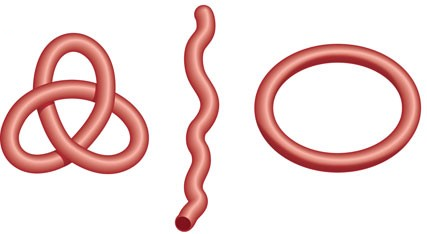
\includegraphics[width=0.8\textwidth]{images/fig1-1.png} 
    \caption{拓扑相变的直观说明。三叶结(左)和简单环(右)分别代表不同的绝缘材料:三叶结是拓扑绝缘体而简单环是普通绝缘体。由于无法通过连续变形将一种形状转变为另一种,因此在两者之间的过渡必须有一个表面,这个表面可以被视为“被切断的结”。\cite{d1}}
    \label{fig_1_1}
\end{figure}


\subsection{量子霍尔效应}
量子霍尔效应(Quantum Hall Effect)是凝聚态物理中最重要的拓扑现象之一,由Klaus von Klitzing于1980年首次发现\cite{d2}(如图\ref{fig_1_2}所示)。这一效应是在二维电子气系统中通过实验观察到的:当强磁场垂直作用于二维导体表面,并且系统处于低温条件下时,霍尔电导呈现完全量子化的特性。其值由公式
\begin{equation} \label{eq1-1}
    \sigma_{xy} = \frac{e^2}{h} n
\end{equation}
确定,其中 \( e \) 是电子电荷,\( h \) 是普朗克常数,\( n \) 是一个整数,称为拓扑不变量。霍尔电导的量子化表明其对材料的微观细节或杂质分布不敏感,而由系统的拓扑性质决定。

这一现象的理论基础是电子在磁场中运动时形成的朗道能级,其能量为:
\begin{equation} \label{eq1-2}
    E_n = \hbar \omega_c \left( n + \frac{1}{2} \right),
\end{equation}
其中 \( \hbar \) 是约化普朗克常数,\( \omega_c = \frac{eB}{m} \) 为回旋频率,\( n \) 是朗道能级的量子数。这些离散能级限制了电子在二维平面中的运动,使得系统的输运性质呈现量子化行为。

1982年,Thouless、Kohmoto、Nightingale和Nijs(TKNN)将整数量子霍尔效应与拓扑不变量联系起来\cite{d3}。他们发现,霍尔电导的量子化可以通过布里渊区中电子态的几何特性来解释,并提出了以下公式:
\begin{equation} \label{eq1-3}
    \sigma_{xy} = \frac{e^2}{h} \frac{1}{2\pi} \int_{BZ} \Omega(\mathbf{k}) \, d^2k,
\end{equation}
其中 \( \Omega(\mathbf{k}) \) 是贝里曲率,表示为贝里联络的旋度。贝里联络的定义为:
\begin{equation} \label{eq1-4}
    \mathbf{A}(\mathbf{k}) = i \langle u(\mathbf{k}) | \nabla_{\mathbf{k}} | u(\mathbf{k}) \rangle,
\end{equation}
这里 \( |u(\mathbf{k})\rangle \) 是布里渊区中的周期波函数。TKNN工作首次明确了霍尔电导的拓扑起源,并将陈数 \( C \) 引入这一框架:
\begin{equation} \label{eq1-5}
    C = \frac{1}{2\pi} \int_{BZ} \Omega(\mathbf{k}) \, d^2k,
\end{equation}
这个整数拓扑不变量直接决定了量子霍尔效应中的量子化电导。

1984年,迈克尔·贝里(Michael Berry)提出了贝里相(Berry Phase)的理论\cite{d4},这是一个与路径相关的几何相位,系统的波函数在参数空间中演化时会积累这一相位。贝里相为理解电子态的几何和拓扑特性提供了基础,贝里联络和贝里曲率的引入进一步深化了对拓扑效应的描述。

1988年,Haldane在以上工作的基础上提出了陈绝缘体(Chern Insulator)的理论\cite{d5}。他设计了一个二维模型,其中通过引入周期性磁通破坏时间反演对称性,使得系统可以在无外加磁场的条件下表现出量子化霍尔效应。陈绝缘体的电导仍然由陈数 \( C \) 确定,但其拓扑特性完全由晶格的能带结构决定,而不依赖于外部磁场。这一模型不仅验证了量子霍尔效应的拓扑本质,也为非磁性拓扑材料的研究奠定了理论基础。

量子霍尔效应及其拓展模型如陈绝缘体,揭示了凝聚态物理中拓扑学与电子输运之间的深刻联系。这些工作从实验发现到理论突破,构建了一个将几何、拓扑与物理现象结合的完整框架,为后续拓扑物质的研究铺平了道路。

\begin{figure}[h!]
    \centering
    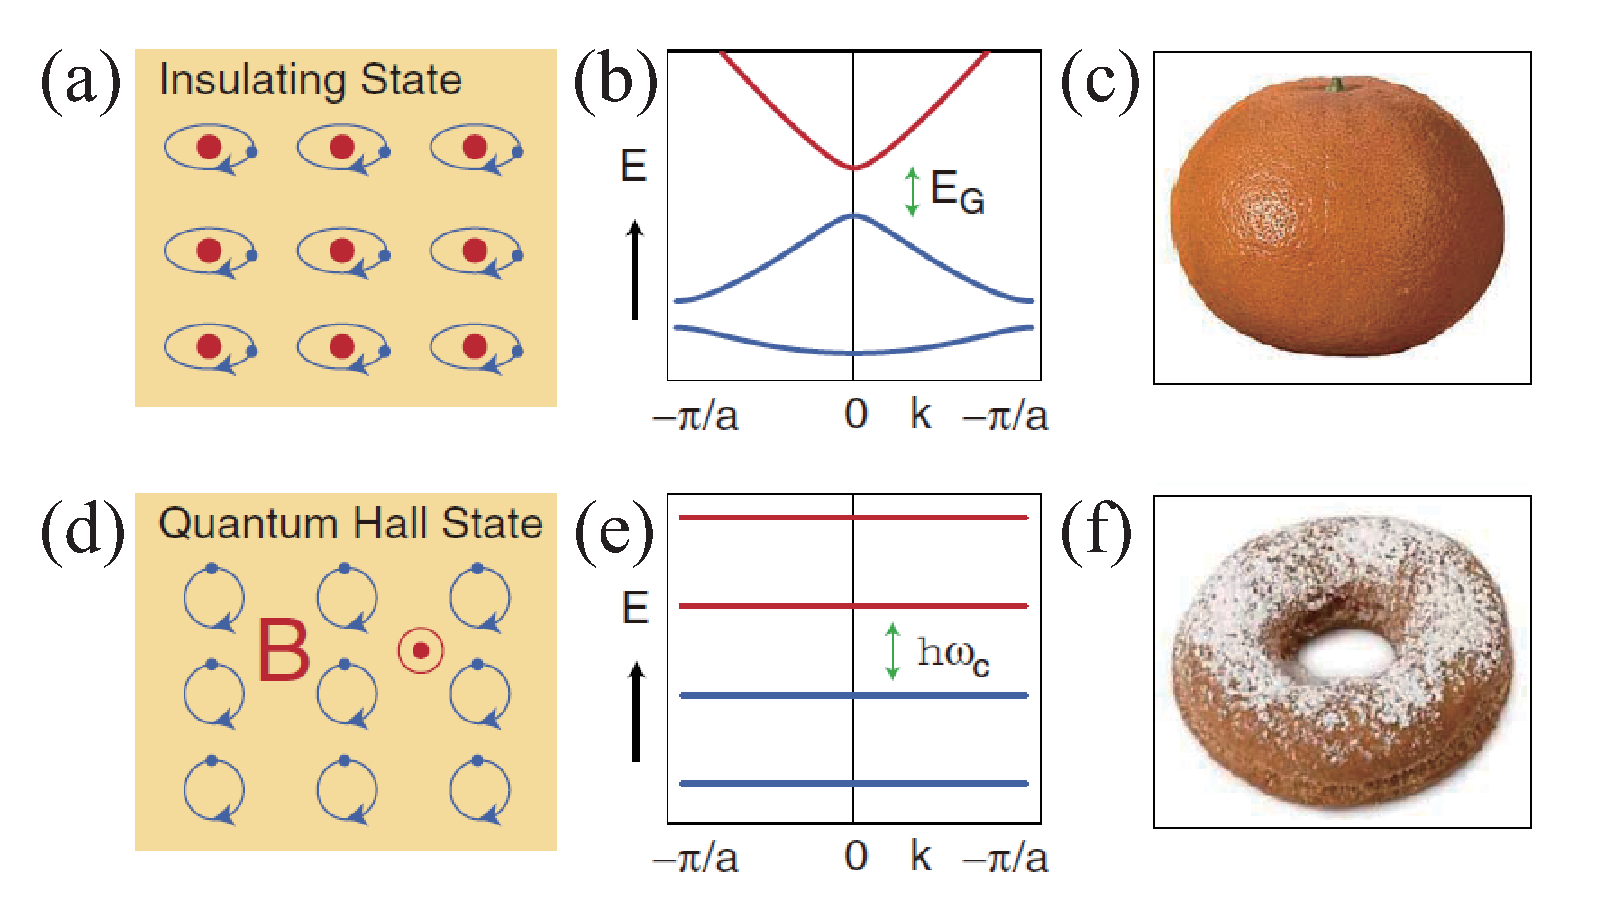
\includegraphics[width=1\textwidth]{images/fig1-2.eps} 
    \caption{量子霍尔效应的说明:(a) 原子绝缘体状态;(b) 简单的绝缘体能带结构;(c) 表示绝缘体的球面(亏格 \( g=0 \))。(d) 量子霍尔态,表现为电子在磁场 \( B \) 中的回旋运动;(e) 朗道能级,显示为离散的能带结构,对应量子化的电子状态;(f) 表示量子霍尔态的圆环形面(亏格 \( g=1 \))。\cite{r11}}
    \label{fig_1_2}
\end{figure}


\subsection{量子自旋霍尔效应}

\begin{figure}[h!]
    \centering
    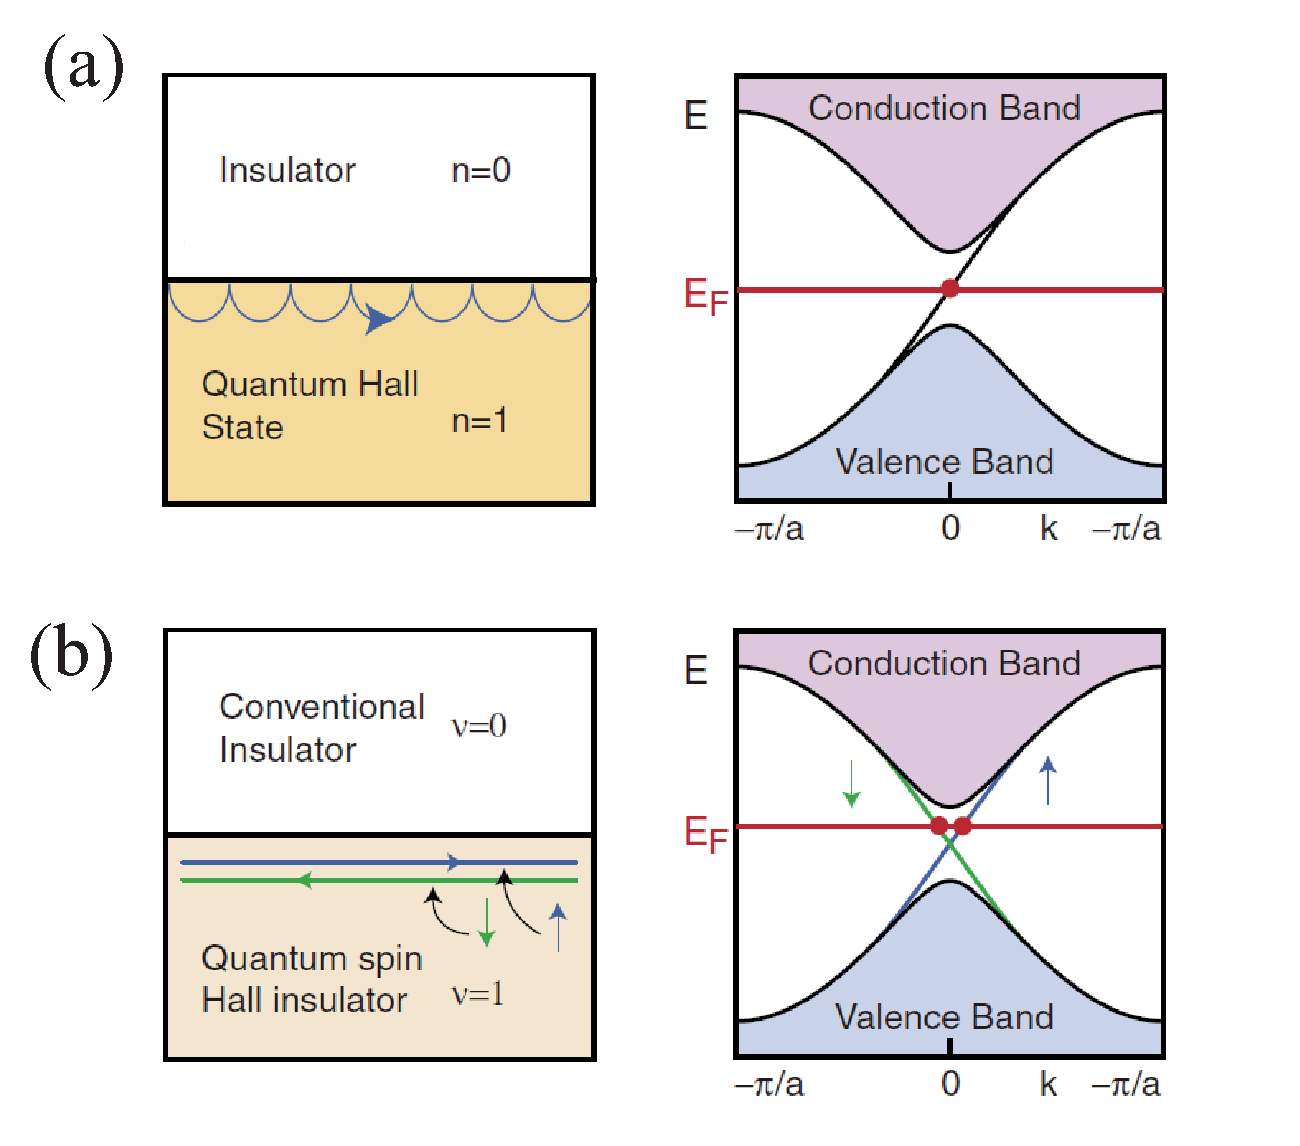
\includegraphics[width=1\textwidth]{images/fig1-3.eps} 
    \caption{量子霍尔效应和量子自旋霍尔效应对比:(a) 量子霍尔效应的边界态和能带结构;(b) 量子自旋霍尔效应的边界态和能带结构。\cite{r11}}
    \label{fig_1_3}
\end{figure}

在量子霍尔效应和陈绝缘体理论的基础上,量子自旋霍尔效应(Quantum Spin Hall Effect, QSHE)作为一种不依赖外加磁场的拓扑量子态逐渐成为研究热点。与传统量子霍尔效应不同,量子自旋霍尔效应通过自旋轨道耦合实现电子自旋与运动方向的联系,从而在系统边缘形成受拓扑保护的无散射传输通道。该效应揭示了非磁性体系中拓扑物态的新特征,并为进一步研究拓扑绝缘体奠定了理论与实验基础。

量子自旋霍尔效应的初步理论框架由Murakami、Nagaosa和Zhang于2004年提出\cite{e1}。他们通过分析具有强自旋轨道耦合的二维电子系统,指出这种耦合会在布里渊区中产生Berry曲率,从而驱动电子表现出类似量子霍尔效应的行为,但其霍尔电导由自旋分量贡献。这一理论表明,自旋向上和自旋向下的电子可以在系统边缘分别沿相反方向传播,而无需外加磁场。

2005年,Kane和Mele进一步扩展了这一理论\cite{e2,e3},提出了自旋霍尔绝缘体的Z₂拓扑不变量,用于描述二维体系中量子自旋霍尔效应的稳定性和边缘态的拓扑保护。在量子自旋霍尔绝缘体中,由于不同自旋分量对应的能隙方向相反,一个外加的电场会分别在自旋向上和向下的电子中感应出相反方向的电流,这导致体系中形成自旋电流,其具体形式为:
\begin{equation} \label{eq1-6}
    J_s = \frac{\hbar}{2e}(J_\uparrow - J_\downarrow),
\end{equation}
其中 \(J_\uparrow\) 和 \(J_\downarrow\) 分别表示自旋向上和向下电子的电流密度。这种自旋电流的存在体现了量子自旋霍尔效应的核心特征,其自旋霍尔电导由以下公式量化:
\begin{equation} \label{eq1-7}
    \sigma_{xy}^s = \frac{e}{2\pi},
\end{equation}
该公式表明,自旋霍尔电导是一个量化的值,与体系中的拓扑性质直接相关。这一工作为理解量子自旋霍尔效应中的拓扑保护机制提供了重要的理论基础,并通过自旋电流和自旋霍尔电导的量化公式进一步揭示了其物理实质。

2006年,Bernevig、Hughes和Zhang预测了一个实际的量子自旋霍尔效应体系——HgTe/CdTe量子阱结构\cite{e4}。当量子阱的厚度超过临界值时,体系会发生拓扑相变,进入量子自旋霍尔态。这一理论预测在König等人的实验中得到了验证\cite{e5}。他们通过低温输运实验发现,这种体系的边缘态表现出无散射传输和量子化导电的特性,即便在没有外加磁场的条件下亦是如此。

量子自旋霍尔效应的拓扑特性由Z₂拓扑不变量决定,反映了系统布里渊区中能带结构的几何特征。与传统量子霍尔效应的整数拓扑不变量(如陈数)不同,Z₂不变量强调体系的时间反演对称性,使其特别适用于非磁性系统的描述。量子自旋霍尔效应不仅拓展了拓扑物理的研究范围,也为拓扑绝缘体、拓扑超导体等新型物态的研究开辟了道路。


\subsection{拓扑晶体绝缘体和高阶拓扑态}

\begin{figure}[h!]
    \centering
    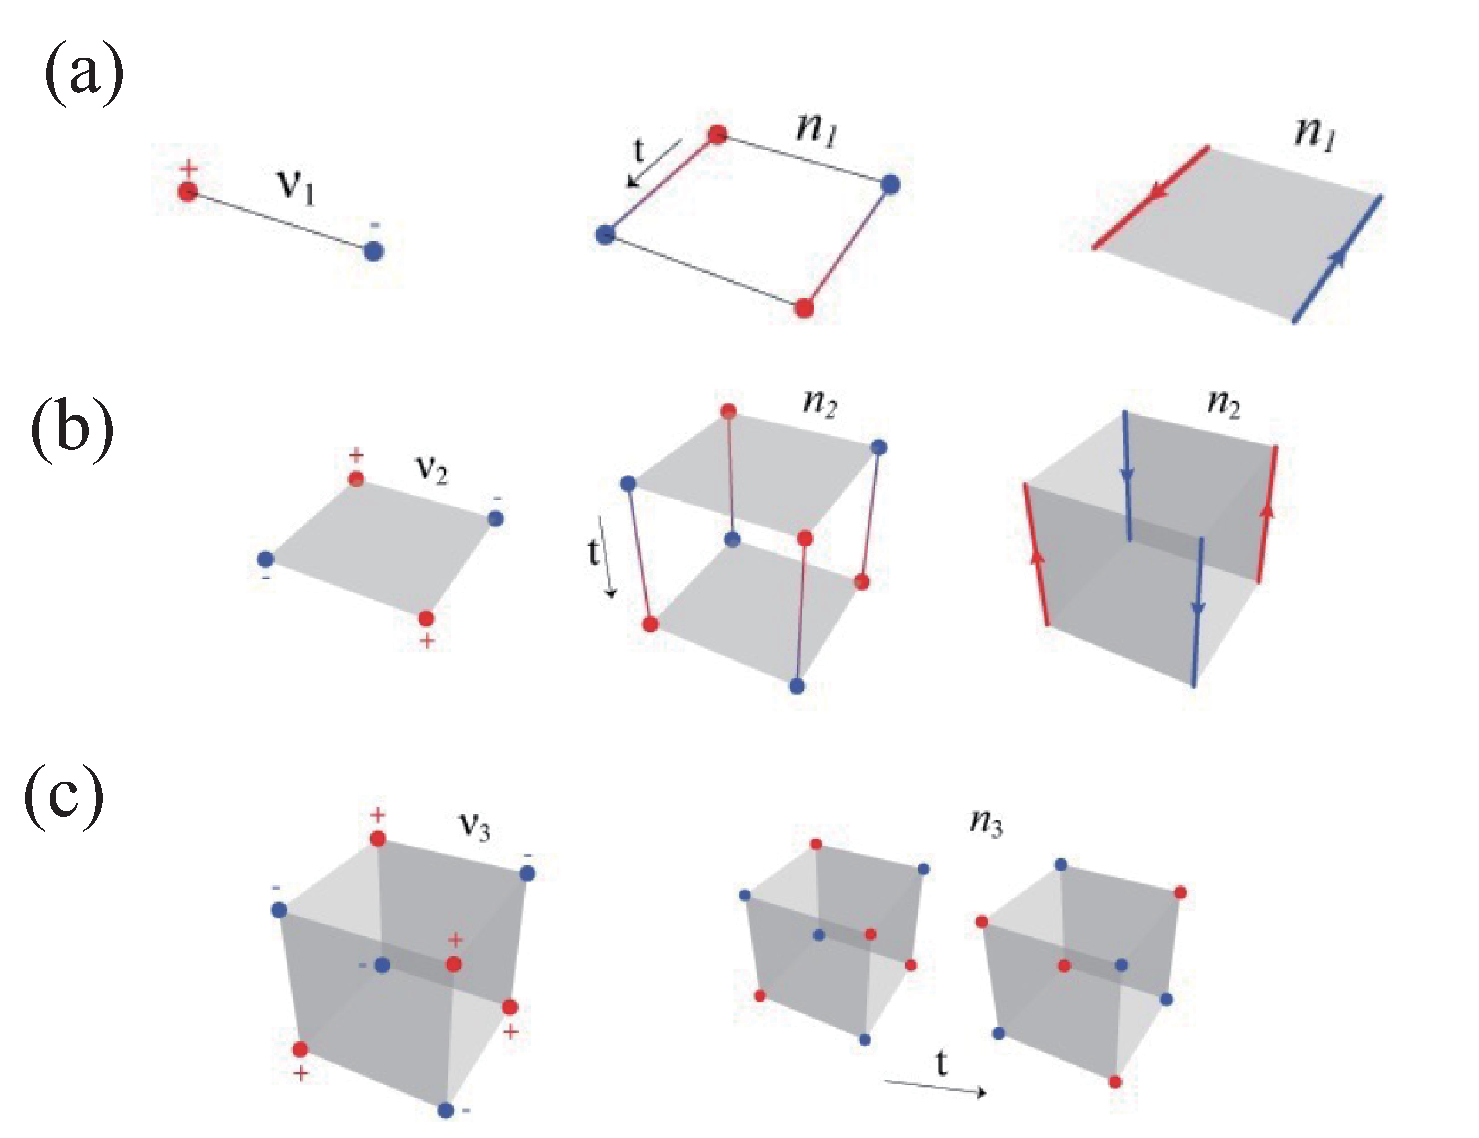
\includegraphics[width=1\textwidth]{images/fig1-4.eps} 
    \caption{多极矩、多极泵浦过程及其衍生的拓扑绝缘体:
    (a) 偶极绝缘体,偶极绝缘体对应的电荷泵浦以及手性边界的局域模态
    (b) 四极绝缘体,四极绝缘体对应的偶极泵浦及其铰链边界的局域模态
    (c) 八极绝缘体及其对应的四极泵浦。
    当受到对称性保护时,电荷量被量化为0或±e/2,并由Z₂拓扑指标ν₁、ν₂和ν₃表示。
    由Chern数n₁、n₂和n₃描述非平凡的闭合循环进行泵浦,会输送电荷、偶极和四极量子\cite{f6}。
    }
    \label{fig_1_4}
\end{figure}

在量子霍尔效应和量子自旋霍尔效应中,时间反演对称性被认为是实现特定拓扑态的关键因素。然而,自然界中晶体材料的空间对称性(如镜面对称性、旋转对称性等)广泛存在。那么受对称性保护的拓扑态能否出现在这些体系中呢?这一问题促使研究者将视角从时间反演对称性拓展到更一般的对称性保护拓扑态,从而引出了拓扑晶体绝缘体(Topological Crystalline Insulator, TCI)的概念。

对于理解高阶拓扑绝缘体的现象而言,核心在于通过多极矩拓扑理论解释更低维度的边界导电现象。传统拓扑绝缘体的特征是体绝缘但边界导电,导电态通常局限于低一维的边界,例如二维材料的边缘或三维材料的表面,而高阶拓扑绝缘体则进一步探讨具有高阶多极矩(如偶极、四极、八极矩)的系统,这些系统的边界态呈现为更低维的导电特性,例如二维系统中的角点态或三维系统中的铰链态(如图\ref{fig_1_4})。2011年,Liang Fu首次提出\cite{f1}。不同于传统的时间反演对称性保护的拓扑绝缘体,TCI的拓扑性质由晶体的镜面对称性和旋转对称性等空间对称性保护。这种拓扑保护使得TCI在晶体的高对称面上能够存在受保护的表面态。例如,Hsieh等人通过第一性原理计算,发现SnTe材料中存在镜面对称性保护的表面态,这些表面态分布在高对称面(如{001}和{111}面)上\cite{f2}。这些表面态的拓扑特性与体系的晶体对称性紧密相关,若镜面对称性被破坏,这些表面态可能退化或消失,这凸显了晶体对称性在TCI中的重要作用。

TCI的理论框架在随后的研究中得到了扩展,特别是在高阶拓扑绝缘体(Higher-Order Topological Insulator, HOTI)的研究中展现了更加丰富的物理现象\cite{f3}。Benalcazar等人提出了基于多极矩描述的HOTI理论,指出高阶拓扑特性不仅表现在二维的表面,还可以出现在一维边界甚至零维角落。例如,在具有Cn旋转对称性的晶体中,其角落电荷可以通过以下公式描述:
\begin{equation} \label{eq1-8}
    Q_{\text{corner}} = \frac{e}{n},
\end{equation}
其中 \(n\) 是旋转对称性的阶数,\(Q_{\text{corner}}\) 是量子化的角落电荷。这一理论进一步揭示了角落电荷的分数化性质,其量子化特性是由系统的对称性和能带结构共同决定的。

Schindler等人通过研究铋(Bi)材料,进一步揭示了三维HOTI的物理特性\cite{f4}。他们发现,铋在边界上的二维表面表现为绝缘体,而在角落处表现为受拓扑保护的局域化态。这种局域化态来源于填充异常(filling anomaly),即能带中电子数与晶体对称性要求的电子数之间的不匹配。填充异常的数学本质可以通过Wannier中心与晶格位置的不匹配来解释。Wannier中心的分布决定了体系的高阶拓扑特性,并与角落电荷的分数化直接相关。

TCI的拓扑特性还可以通过布里渊区中的拓扑不变量来量化。例如,体系的晶格极化可以用以下公式定义:
\begin{equation} \label{eq1-9}
    P^{(n)} = p_1 a_1 + p_2 a_2,
\end{equation}
其中 \(P^{(n)}\) 表示晶体的极化,\(p_1\) 和 \(p_2\) 是布里渊区中不可缩环上的Berry相位,\(a_1\) 和 \(a_2\) 是晶格的基矢量。通过这一公式,可以预测高阶TCI中的角落态和边界态的分布。

此外,Slager等人通过分析空间群的对称性,系统性地分类了不同的拓扑绝缘体\cite{f5}。他们提出了一种基于空间群对称性的拓扑绝缘体分类方法,将TCI与晶体的对称性紧密联系在一起。这一分类方法不仅适用于传统的TCI,还能够描述高阶拓扑绝缘体的拓扑特性,从而为拓扑物态的理论研究提供了完整的框架。

TCI的研究为拓扑物态的理解提供了新的视角,不仅揭示了晶体对称性如何影响拓扑特性,还为设计具有特定拓扑性质的材料提供了理论依据。这些研究在理论和实验上均取得了显著进展,并为未来探索更复杂的拓扑物态奠定了基础。 


\section{电磁波系统中寻找类拓扑效应}

\begin{figure}[h!]
    \centering
    \includegraphics[width=1\textwidth]{images/fig1-5.eps} 
    \caption{使用光子晶体构造类陈绝缘体\cite{g2}:
    (a) 波导的示意图:该波导由一块的光子晶体板(蓝色柱状结构)和金属壁(黄色部分)组成。整个结构被夹在两块平行的铜板(黄色)之间,以限制波导在 \( z \) 方向的传播,并被微波吸收泡沫(灰色区域)包裹。
    (b) 计算得到的场分布(颜色标度)显示了手性边界态如何绕过障碍物传播:波正向传播时能绕过散射体,并且背向传播被抑制
    (c) 光子晶体中测得的前向(蓝线)和后向(红线)传输谱。
    }
    \label{fig_1_5}
\end{figure}

\begin{figure}[h!]
    \centering
    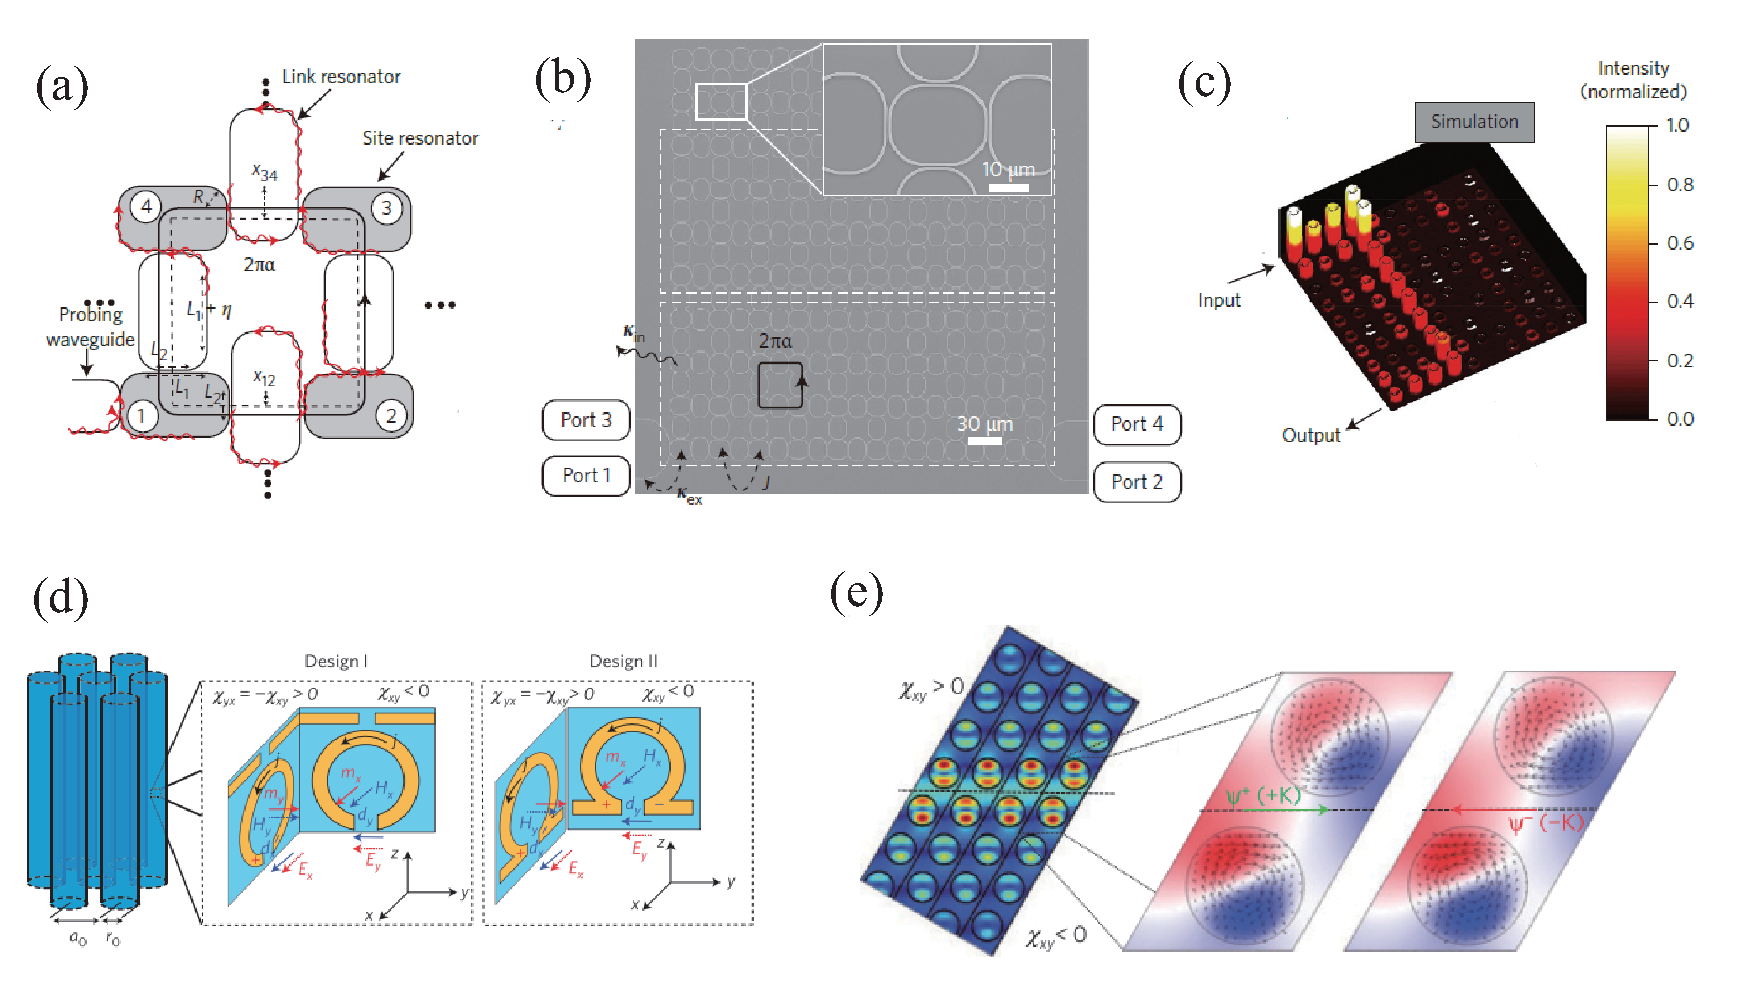
\includegraphics[width=1\textwidth]{images/fig1-6.eps} 
    \caption{使用光子晶体构造量子自旋霍尔效应:
    (a-c) 利用环形谐振腔阵列产生了类似于电子自旋与轨道耦合的现象\cite{g2}:(a) 单元环形谐振腔结构, (b) 单元周期排列结构, (c) 模拟得到的边界态。
    (d-e) 通过光子晶体的TE+TM和TE-TM模式构造赝自旋\cite{g-add-1}:(d) 双向各向异性结构,(e) 上自旋和下自旋的螺旋形边界态。
    }
    \label{fig_1_6}
\end{figure}

由于波动方程的相似性,电磁波作为经典波动形式,近年来通过引入拓扑物理学的核心概念,展现出许多奇异的物质拓扑相位现象,开辟了新的研究方向。经典波系统中的拓扑绝缘体是通过构造具有特定对称性和拓扑特征的波导或晶体结构来实现的。这些系统的拓扑性质使得它们在边界或表面上支持无反射的边界态,展现出独特的物理现象。

Haldane 和 Raghu 在 2008 年首次提出了光子晶体中的类量子霍尔效应的拓扑绝缘体模型\cite{g1},展示了如何通过引入非平庸的拓扑相位来实现光子的单向传播(如图\ref{fig_1_5})。这一模型的核心在于,通过引入时间反演对称性破缺的机制,例如磁性光学材料,可以在光子晶体的能带结构中打开拓扑能隙,使得光子的传播方向被拓扑保护。具体而言,光子晶体的周期性结构使得光子的传播特性受到调制,从而形成带隙结构。这种设计允许光子在带隙中只能以单向的形式传播,同时避免了散射和反射的影响。随后,2009 年 Wang 等人成功在实验中验证了这一理论\cite{g2}。他们利用二维磁性光子晶体,在实验中观察到了稳健的单向边界态,这种边界态不仅可以有效防止背向散射,而且在一定程度上对缺陷和杂质不敏感,为光子学中的拓扑物理研究提供了实验支持。

为了在光学领域实现类似于量子自旋霍尔效应的拓扑模型并探索其应用,其中一个主要问题是在光学领域缺乏大的磁光响应。解决这一难题的方法之一是将光子的内部自由度视为类自旋,并寻找类比于量子自旋霍尔系统的模型,即整体时间反演对称性未被破坏,但每个赝自旋感受到人工磁场。2011 年,Hafezi 等人通过在光学系统中引入类似于电子系统中的自旋自由度,提出了一种模拟量子自旋霍尔效应的光学类比模型\cite{g3,g6}。具体而言,他们设计了一种基于环形谐振腔阵列的光学结构(如图\ref{fig_1_6} (a-c)),这种结构通过人为构造的光学路径,产生了类似于电子自旋与轨道耦合的现象(如图\ref{fig_1_6} (a)),从而在光子系统中实现了类自旋霍尔效应。他们的研究表明,自旋自由度的引入可以在光子系统中产生稳健的拓扑边界态,这些边界态不仅能够有效地抵抗缺陷和无序的影响,还能够实现无损耗的单向传播。另一种思路是利用光学偏振模式来等效上自旋和下自旋态。例如,2013年,Khanikaev等人通过设计双各向异性单元,利用了结构中TE+TM和TE-TM两种偏振模式构造赝自旋(如图\ref{fig_1_6} (d-e)),从而实现了光量子自旋霍尔效应\cite{g-add-1}。这种超表面的界面支持螺旋边缘态,这些态表现出光子的自旋极化单向传播,并且受无序性的影响很小。他们的结果表明,无需打破时间反演对称也可实现单向光子传输。

以上关于类量子霍尔效应和类量子霍尔效应被引入到经典波系统之后,研究者们又开始思考能否在经典波系统中观测到高阶拓扑效应。由于高阶拓扑效应的产生可以不依赖时间反演对称的破缺,所以经典波系统中具有空间对称性的周期结构成为了简易实现高阶拓扑的极佳平台。2018年,Peterson等人展示了一种量化微波四极拓扑绝缘体\cite{h5},其使用了耦合微波谐振器阵列构建了二维四极模型,并通过光谱测量验证了其拓扑性和角态的存在(如图\ref{fig_1_7} (a))。此外,通过改变晶格边界从拓扑相到平庸相的转变,实验确认了角态的拓扑保护性。同年,Noh等人飞秒激光直接写入技术制造了一系列波导阵列,形成具有六重对称性和特定拓扑性质的二维结构\cite{h6}。研究显示,这些晶格在拓扑相中支持局限于角落的零模,这些零模的频率稳定于能隙中间,不受结构缺陷的影响(如图\ref{fig_1_7} (b))。

\begin{figure}[h!]
    \centering
    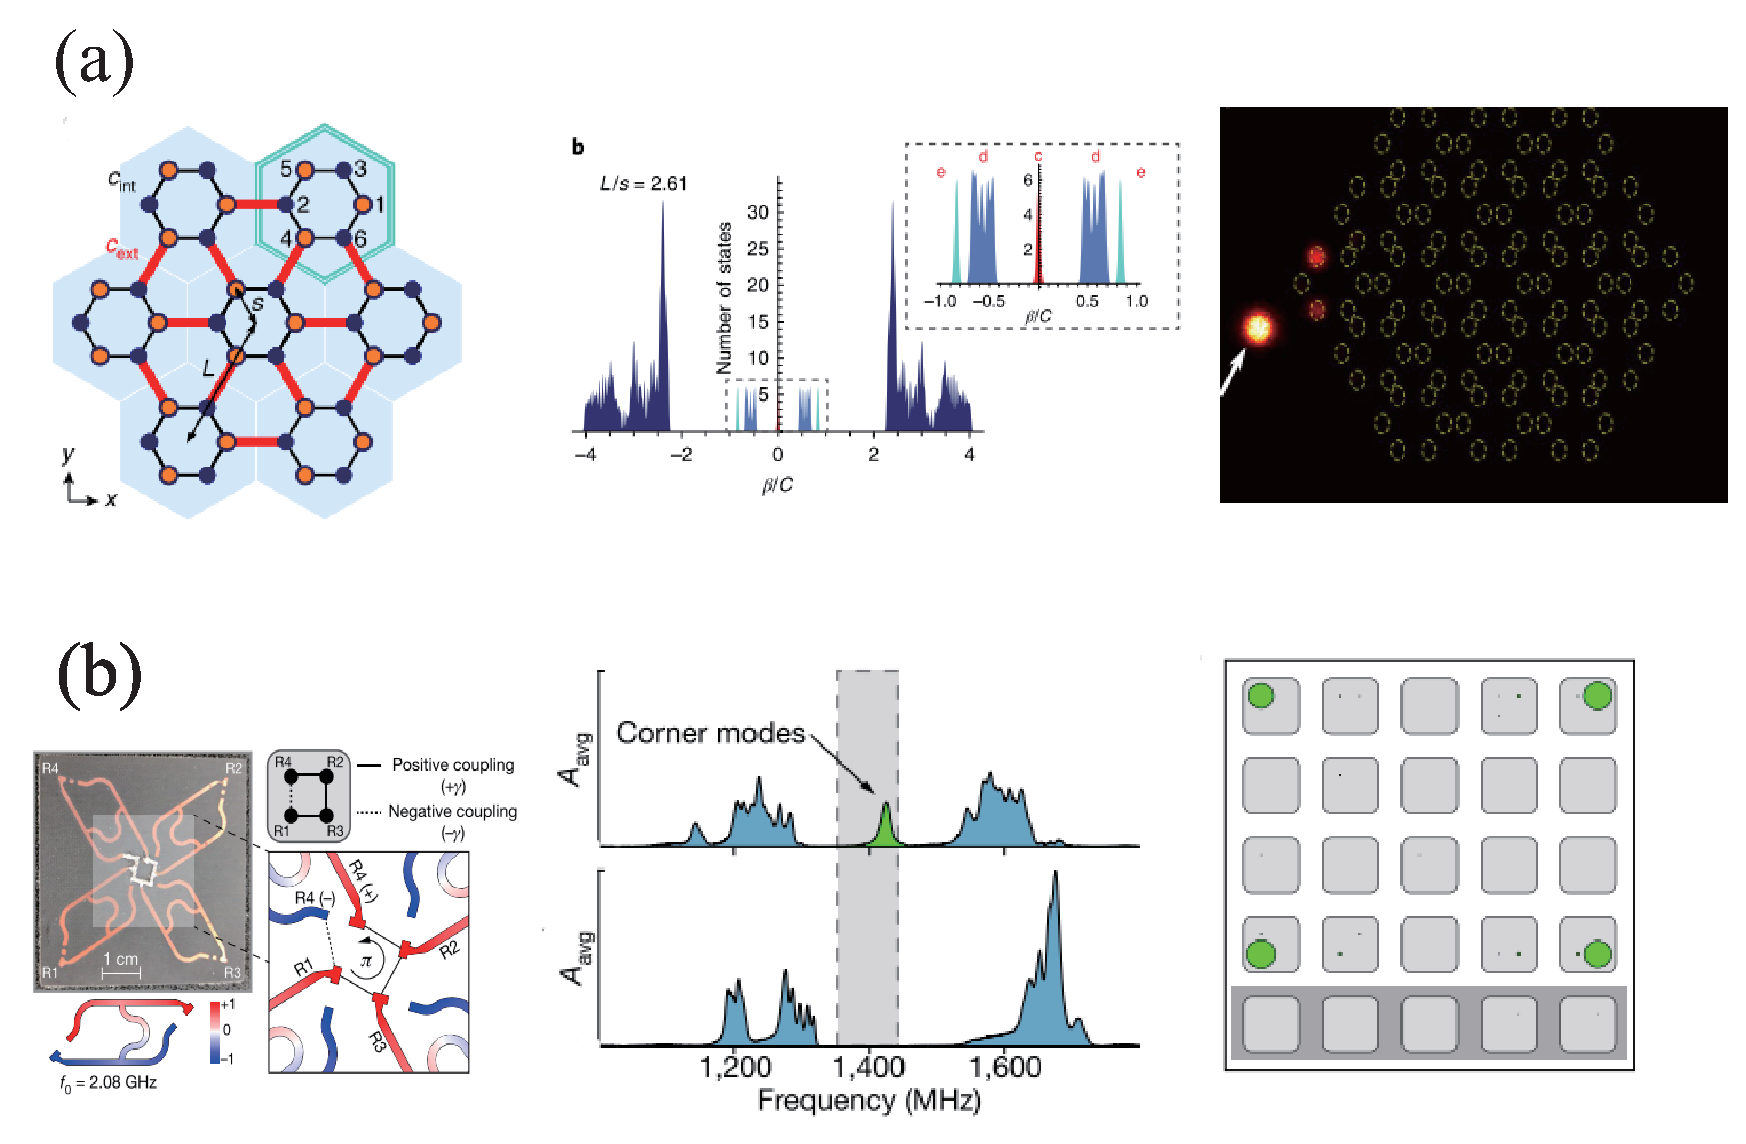
\includegraphics[width=1\textwidth]{images/fig1-7.eps} 
    \caption{光学系统中的高阶拓扑现象:
    (a) 具有$C_6$对称性的光学高阶拓扑绝缘体\cite{h5},从左到右分别为结构图,态密度图和实验观测到的高阶拓扑模态。(b) 微波四极绝缘体\cite{h6},从左到右分别为结构图,态密度图和实验观测到的高阶拓扑模态。
    }
    \label{fig_1_7}
\end{figure}

除此之外,许多丰富且深刻的拓扑效应在电磁波平台上得以实现。例如在Floquet拓扑绝缘体的理论基础上\cite{g4,g5},通过时间周期性的外部调制,使系统形成一个有效的时间无关哈密顿量,从而实现时间反演对称性的动态破缺。这一理论从凝聚态物理中延伸至光学系统,并在2013年由Rechtsman等人通过设计二维波导阵列系统,观察到了与Floquet拓扑绝缘体相关的单向边界态\cite{g7}。此外,另一种基于时间依赖性调制的方式,即“拓扑泵”理论\cite{g8},通过对系统施加时间演化的调制,可以实现量子态的拓扑保护转移。这一方法最终在2012年由Kraus 等通过实验验证,他们成功实现了基于光子学的拓扑泵现象,进一步丰富了光学拓扑物理的实验体系\cite{g9}。这些理论与实验的结合,不仅推动了光学系统中拓扑效应的深入研究,也为未来开发新型光学器件提供了理论指导和实践支持\cite{h1,h2,h3,h4,h7,h8,h9,h10,h11,h12,h13,h14,h15,h16}。


\section{声学拓扑绝缘体的研究现状}

声学和光学在波动特性上具有显著的相似性,两者均可以通过波动方程进行描述,并且其传播行为如反射、折射和干涉等基本现象具有一致的物理机制。此外,声学系统和光学系统都可以通过人工设计的周期性结构(例如光子晶体和声子晶体)调控波的传播特性,例如实现能带结构和带隙特性,从而引入拓扑物理的相关概念。基于这一类比,光学拓扑系统的研究为声学拓扑绝缘体的实现提供了重要的理论借鉴,特别是在通过晶格对称性破缺引入拓扑保护态和能带倒转等方面。与此同时,声学拓扑绝缘体在实现方式上由于声波的长波长特性,往往较光学系统更为灵活,适用于更宽的频率范围,因而在工程应用中具有独特的优势。这种物理上的相似性和技术上的互补性,使得声学拓扑绝缘体成为研究的热点领域之一。

\subsection{声学类量子霍尔效应}

\begin{figure}[h!]
    \centering
    \includegraphics[width=1\textwidth]{images/fig1-8.eps} 
    \caption{声学系统中的陈绝缘体:
    (a) 通过环形流场环绕的周期性圆柱阵列构造声学陈绝缘体。(b) ribbon排列的超元胞能带结构。(c) 沿着界面单向传播的声学边界态的声场分布。(d) 声学陈绝缘体的实验装置\cite{i-add-1},(e)背景流场分别为$10\pi$ rad/s 和$-10\pi$ rad/s 的声传输实验结果。
    }
    \label{fig_1_8}
\end{figure}

相较于光学系统,在声学系统中打破时间反演对称并不是一件容易的事情。2015年,Yang等人首次提出并验证了声学陈拓扑绝缘体的实现方案\cite{i1},该方案基于循环流体的声学晶格,成功生成了无反向散射的单向声波传播边界态,如图\ref{fig_1_8}。与传统声学器件不同,此类边界态受拓扑保护,具有对缺陷和无序的鲁棒性。作者借助含有循环流体的声学晶格结构,通过有限元数值计算首次证明了此类声学系统具有非零陈数的声学能带。具体而言,研究人员设计了一种三角形晶格结构,其中每个晶格单元由金属柱与围绕其旋转的环形流体组成。声波在这个体系中控制方程可化简为:
\begin{equation} \label{eq1-10}
    \left[ (\nabla - i \vec{A}_{\text{eff}})^2 + V(x, y) \right] \Psi = 0,
\end{equation}  
其中,$\Psi = \sqrt{\rho} \phi$,$\rho$为流体密度,$\phi$为速度势。旋转流体在晶格中产生类磁场效应,方程中有效矢量势和标量势的表达式分别为:  
\begin{equation} \label{eq1-11}
    \vec{A}_{\text{eff}} = -\frac{\omega \vec{v_0}(x, y)}{c^2}
\end{equation}
\begin{equation} \label{eq1-12}
    V(x, y) = -\frac{1}{4} \left|\nabla \ln \rho\right|^2 - \frac{1}{2} \nabla^2 \ln \rho + \frac{\omega^2}{c^2}
\end{equation}
其中,\(\omega\) 是角频率。背景流场的速度$v_0$分布决定了矢量势的空间变化。
背景流场的存在破坏了时间反演对称性,从而打开了Dirac点处的能隙,生成了具有拓扑保护特性的声学边界态。能隙内存在单向传播的声学边界态具有与量子霍尔效应中电子边界态类似的特性,即单向传播且不受散射影响。研究表明,体系中的拓扑边界态具有强鲁棒性。例如,声波能够在包含90度和180度弯折的边界路径中无损通过,且在接触声腔时仅激发局域共振而不会反向散射。而在2019年,Ding等人首次在声学系统中实验实现了陈绝缘体\cite{i-add-1}。他们通过使用具有角动量偏置的谐振器阵列来打破洛伦兹互易性。其中,谐振器的高品质因子共振被用来降低所需的旋转速度,并构造了等效的磁场。实验结果表明,声学陈绝缘体在稳定和均匀的超流体流动偏置下,能够支持声波在边缘的单向非互易传输,并且这种传输拓扑上能够免疫于各种类型的缺陷。

\subsection{声学类量子自旋霍尔效应}

\begin{figure}[h!]
    \centering
    \includegraphics[width=1\textwidth]{images/fig1-9.eps} 
    \caption{声学系统中的类量子自旋霍尔效应\cite{i2}:
    (a) 不同填充率的类石墨烯排布的声子晶体的结构图。(b) ribbon排列的超元胞能带结构。(c) 不同路径的声传输实验结果。
    }
    \label{fig_1_9}
\end{figure}

声学陈绝缘体通过时间反演对称性破缺实现了单向传播的声学边界态,但通常依赖于外部动力学调制或循环流体,这些限制了其实用性和广泛应用的可能性。为解决这一问题,He等人提出无需时间反演对称性破缺的声学量子自旋霍尔效应的实现方式,通过几何设计引入赝自旋自由度\cite{i2}。研究采用了一种由不锈钢圆柱排列在空气中构成的类石墨烯结构的声子晶体,通过调整圆柱半径与晶格常数的比值(即填充因子),在布里渊区中心形成了四重简并的双重狄拉克锥,如图\ref{fig_1_9}。这种双重狄拉克锥的构建基于$C_{6v}$对称性下的能带耦合机制。具体而言,为引入实现声学量子自旋霍尔效应的赝自旋,这种特殊的对称性结构的通过混合$p_x/p_y$和$d_{x^2-y^2}/d_{xy}$的声学模态构建出赝自旋$+/-$模态,它们分别定义为$p_{\pm} = (p_x\pm ip_y)/\sqrt{2}$和$d_{\pm} = (d_{x^2-y^2}\pm id_{xy})/\sqrt{2}$。赝自旋的引入为声波提供了类似电子系统中自旋的自由度,使得在拓扑声子晶体与普通声子晶体界面处能够形成受拓扑保护的边界态。边界态由对称模态(S)和反对称模态(A)混合构成,分别对应于$S+iA$和$S-iA$,从而展现出显著的自旋依赖性。当填充因子逐步减小时,系统经历了拓扑相变,能带顺序发生倒转,从普通声子晶体转变为拓扑声子晶体。这一相变过程清晰地反映了几何设计对能带结构的调控作用和拓扑性质的改变。这种机制使得边界态的传播方向由伪自旋态决定,确保了单向传播的性质。

实验进一步验证了伪自旋依赖的单向边界态传播特性,如图\ref{fig_1_9} (c)。研究设计了一种交叉波导分离器,用于激发和检测不同伪自旋态下的声波传输行为。实验结果显示,当输入声波具有特定伪自旋态时,声波仅能沿预定方向传播,而另一伪自旋态的传播被完全抑制。此外,这些边界态对缺陷(如腔体、无序和弯曲路径)表现出显著的鲁棒性。例如,在存在复杂边界条件的情况下,声波能够绕过缺陷实现高效传输,且传播特性几乎不受影响。尤其是在带隙内的频率范围内,声波的传输效率保持稳定,这表明拓扑边界态具有良好的缺陷免疫能力。

\subsection{声学谷霍尔效应}

\begin{figure}[h!]
    \centering
    \includegraphics[width=1\textwidth]{images/fig1-10.eps} 
    \caption{声学系统中的谷霍尔效应\cite{i3}:
    (a) 三角形排列的刚性柱晶格的声学谷霍尔绝缘体的结构图。(b) 周期结构能带结构和拓扑相变。(c) 边界态声传输的声场分布的实验结果。
    }
    \label{fig_1_10}
\end{figure}

除了声学陈绝缘体和声学量子霍尔效应之外,声学谷霍尔效应也是近年来声学拓扑物态研究的重要方向之一,其灵感来源于电子系统中的谷度自由度和谷霍尔效应。谷霍尔效应指的是在晶格对称性被破坏的情况下,电子在布里渊区的两个谷(通常指布里渊区中能带极值处的动量空间区域)中表现出相反的轨道磁矩和电导行为,这种效应被成功地迁移到声学系统中,为声波传播控制提供了全新的机制。与电子相比,声波缺乏电荷和自旋等内禀自由度,然而通过几何设计和人工构造的拓扑晶格,可以在声学系统中实现类似谷自由度的物理现象。声学谷霍尔效应的核心在于通过破坏晶格的空间对称性(例如镜面对称性或旋转对称性),在布里渊区的两个谷中诱导相反的拓扑性质,从而形成声波的谷极化(valley polarization)。这意味着声波可以根据其所在谷的不同,以特定的方式传播。这种机制无需时间反演对称性破缺,相比传统的声学陈绝缘体和量子自旋霍尔效应,其实现难度显著降低。

2017年,Lu等人基于二维声子晶体的设计,首次通过实验验证了声学谷霍尔效应的存在及其拓扑保护特性\cite{i3}。他们的研究以二维三角形排列的刚性柱晶格为基础,利用调整晶格单元的几何参数实现对称性的破坏,从而在布里渊区的K点和K'点打开能隙,形成谷态,如图\ref{fig_1_10}。通过Floquet-Bloch理论分析,这一系统的声学能带结构在布里渊区的K点和K'点附近表现为Dirac锥。当通过旋转刚性柱以破坏镜面对称性时,Dirac锥的简并被解除,能带在K点和K'点打开带隙。这一现象可通过一个有效的哈密顿量描述:
\begin{equation} \label{eq1-13}
    H_{\text{eff}} = v_F (\tau_z k_x \sigma_x + k_y \sigma_y) + m \sigma_z,
\end{equation}
其中,\(v_F\) 是等效的声波传播速度,\(k_x\) 和 \(k_y\) 为动量分量,\(\sigma_i\) 为Pauli矩阵,\(\tau_z = \pm 1\) 表示K和K'谷态,\(m\) 是质量项,其值和符号由镜面对称性破缺的程度决定。通过对贝里曲率的积分,可以计算谷Chern数,用以表征两个谷态的拓扑性质:
\begin{equation} \label{eq1-14}
    \mathcal{C}_v = \frac{1}{2\pi} \int_{\text{BZ}} \nabla \times \mathbf{A} \, d^2k,
\end{equation}
其中,\(\mathbf{A} = i \langle u_k | \nabla_k | u_k \rangle\) 是贝里联络,\(u_k\) 为布里渊区内的能带本征态。Lu等人通过调节三角柱的旋转角度,使得不同区域的谷Chern数分别为\(+1\)和\(-1\),从而在两域的界面处形成拓扑保护的单向传播边界态。

为了验证理论的准确性,他们采用周期性排列的三角形刚性柱,并通过调整三角柱的旋转角度控制对称性破缺程度,从而生成不同的谷态域。在两个谷态域的界面处,Lu等人通过高斯波束激励声波,并测量了界面上的声波传播特性。结果显示,界面处的声波能够沿单一方向传播,即使在界面存在尖角、弯曲或缺陷时,声波的传播行为仍保持稳定。此外,实验还通过改变高斯波束的入射角,观察了特定谷态的选择性激发现象,不同的入射角可以选择性地激发特定的K或K'谷态边界声波,验证了声学谷霍尔效应的谷态选择特性。以上的实验结果与理论分析和数值模拟高度一致:理论预测的拓扑保护边界态表现为单向传播,具有很高的鲁棒性,而实验中声波在经过尖锐的弯曲路径或无序区域后仍能保持传播方向和能量传输稳定性。这一研究表明,声学谷霍尔效应中的拓扑保护机制能够有效避免常规声波导中的散射损耗,为声波的高效传输提供了新的物理机制。

\subsection{声学高阶拓扑绝缘体}

\begin{figure}[h!]
    \centering
    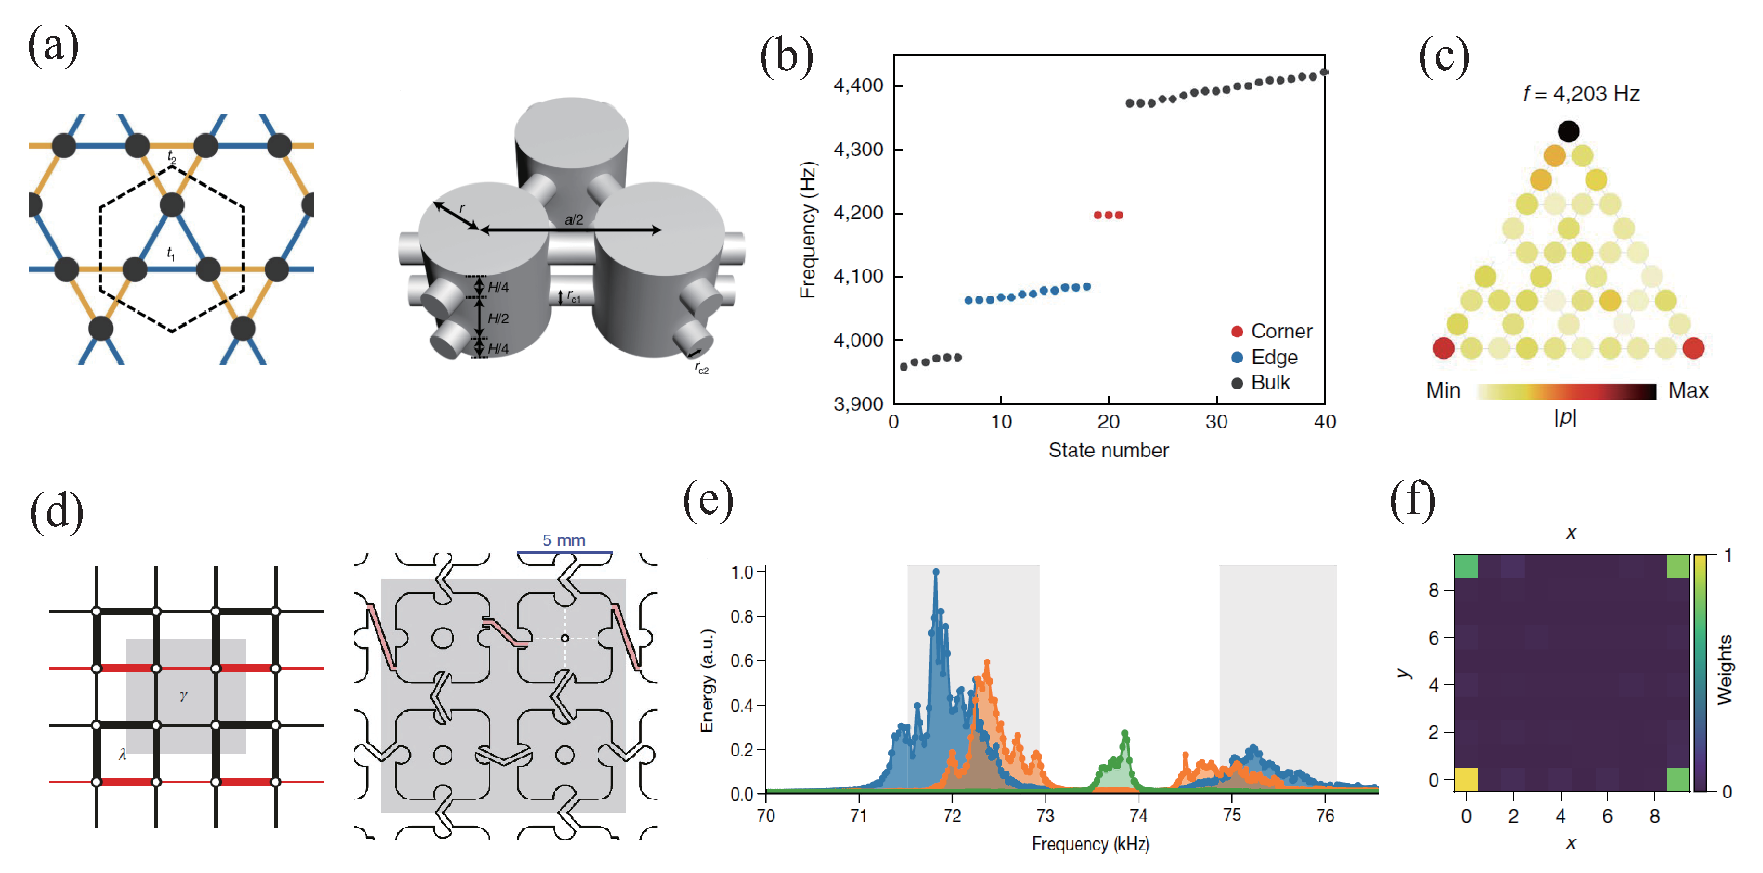
\includegraphics[width=1\textwidth]{images/fig1-11.eps} 
    \caption{声学系统中的高阶拓扑:
    (a-c) Kagome晶格的高阶角态\cite{i4}:(a)Kagome晶格结构,(b)有限大结构的体态,边界态, (c) 角度的声场分布。
    (d-f) 声学四极子高阶拓扑态\cite{i6}: (c)声学四极子结构, (d)有限大结构的体态,边界态和角态的声传输情况, (e)角态的声场分布。
    }
    \label{fig_1_11}
\end{figure}

声学高阶拓扑绝缘体(Acoustic Higher-Order Topological Insulator, HOTI)是近年来声学拓扑物态研究的重要分支,其特征在于拓扑态不仅限于一维边界,还延伸至更高阶维度,如零维角点态或二维面态。相比传统的一阶拓扑绝缘体,高阶拓扑绝缘体展现了更加复杂的几何极化和拓扑保护特性,在理论研究和实验验证方面逐步取得了重要进展。

2018年,Xue等人首次提出声学高阶拓扑绝缘体的理论框架并进行了实验验证\cite{i4}。他们基于Kagome晶格设计了一种二维声学系统,通过对晶格结构的几何调控破坏对称性,在布里渊区打开带隙,从而生成了零维角点局域态。在实验中,他们利用压力场分布的测量,观测到这些角点态的声学局域化特性。理论上,通过几何极化的计算,他们明确了高阶拓扑态与晶格对称性之间的关系。这一研究首次验证了声学高阶拓扑绝缘体的存在,为后续研究奠定了重要基础。随后,Ni等人进一步拓展了声学高阶拓扑绝缘体的设计\cite{i5},他们利用三角对称性的声子晶格,设计了一种周期性排列的声学散射柱阵列,通过几何设计打开拓扑带隙,形成了角点态。这些角点态通过数值计算和实验验证,表现出对缺陷和无序的高度鲁棒性。他们的工作进一步丰富了高阶拓扑绝缘体的几何设计方法,并证明了其在复杂环境中的适应性。

除了Kagome晶格外,研究者在其他对称性结构中观测到了声学高阶拓扑态\cite{i6}。例如,Serra Garcia等人使用硅片构建了一种基于四极矩拓扑理论的声学系统,并首次在实验中观测到了这一新型拓扑态。它们的结构中每个硅片单元通过细梁连接,这些梁的设计确保了系统中的耦合强度具有正负交替的特性,从而在布里渊区形成拓扑带隙。通过超声换能器激励声波,并使用激光干涉仪测量振动模式,研究者在四个角点检测到了局域化的声学态。这些局域态与理论预测一致,表明系统中存在四极矩拓扑保护。通过调整对称性破缺的参数,研究者观察到了拓扑相变的发生,并确认了系统中的拓扑态具有鲁棒性。

2020年,Zhang等人实现了三维声学高阶拓扑绝缘体的实验观测\cite{i7}。他们设计简单立方晶格几何结构的三维声子晶体,通过改变空气腔中心间距实现拓扑相变,并计算其能带结构及拓扑性质确定为三阶高阶拓扑绝缘体。实验上,他们利用光敏树脂3D打印制备制备“表面”“铰链”“角”样品,采用泵浦探测测量技术,对不同样品进行测量和分析,观测到二维表面态、一维铰链态和零维角态,验证了各维度拓扑边界态在带隙中的存在、能量局域特性及对对称保持扰动的鲁棒性,证明了其拓扑特性。

2022年,Gao等人将研究拓展到非厄密条件下的声学高阶拓扑绝缘体\cite{i8}。他们采用了一种基于非厄密 Benalcazar-Bernevig-Hughes (BBH) 模型的理论框架,提出通过精确设计的非均匀损耗分布可以在声学系统中生成具有四极矩拓扑特性的高阶拓扑态。在该模型中,声学单元格由16个谐振器组成,其中谐振器通过不同强度的损耗参数(\(\gamma_1\) 和 \(\gamma_2\))实现非厄密性。具体而言,他们通过在谐振器上打孔并填充吸声材料来调控损耗强度,从而实现非厄密系统的可控性后,通过声学测量体态、边界态以及零维角点态的声压分布,重点研究了角点模式的局域化特性。这些角点态位于系统的带隙内,是非厄密损耗分布驱动形成的四极矩拓扑相的直接体现。此外,通过改变损耗配置,他们进一步观察到了拓扑相的转变。这项工作展示了非厄密损耗在声学晶体中生成高阶拓扑态的作用,实验设计和理论分析为非平衡拓扑系统的研究提供了重要示范。

声学高阶拓扑绝缘体的研究经历了从二维到三维、从静态到动态、从厄密到非厄密系统的多维发展过程。通过几何设计、对称性调控和动态参数调节,研究者逐步建立了声学高阶拓扑态的物理基础,并提出了多种实验验证方法。这些工作不仅深化了对声学拓扑物态的理解,还为基于高阶拓扑特性的声学器件开发提供了理论支持和技术指导,未来的研究将进一步推动高阶拓扑态在更复杂系统中的实现及其实际应用。

\subsection{声学系统中的其他拓扑效应}

\begin{figure}[h!]
    \centering
    \includegraphics[width=1\textwidth]{images/fig1-12.eps} 
    \caption{声学系统中拓扑效应的应用:
    (a) 基于谷霍尔拓扑绝缘体的定向声学天线\cite{j2},(b)基于多谐振声子晶体拓扑边缘态的新型声能收集装置\cite{j17},(c)基于拓扑保护声子模式的新型拓扑声镊\cite{j13}。
    }
    \label{fig_1_12}
\end{figure}

近年来,声学拓扑领域的研究呈现出蓬勃发展态势,众多前沿成果不断涌现,极大拓展了该领域边界。除前文提及的相关研究工作外,当下科研人员围绕声学拓扑开展了更为深入且全面的探索\cite{j1,j2,j3,j4,j5,j6,j7,j8,j9,j10,j11,j12,j13,j14,j15,j16,j17}。一方面,这类研究有力揭示了量子系统与经典物理系统之间的内在关联性。量子系统微观抽象,遵循独特物理规律;经典物理系统相对宏观直观,二者特性迥异。声学平台却以其宏观、易操作的优势,脱颖而出成为验证量子效应的优质选择。在声学体系里,科研人员能利用相对简便的实验装置与操作流程,模拟复杂量子现象,进而洞察量子与经典系统间隐匿的联系纽带,为基础理论的深度融合提供关键支撑。另一方面,声学边界态具有对缺陷的强鲁棒性,无背向散射等特性,使得声学拓扑在声学领域有着广泛而重要的应用,为声学操控和声学研究带来了新的思路和方法,如图\ref{fig_1_12}。例如,Zhang等人基于谷霍尔拓扑绝缘体的提出了一种新的定向声学天线,Zhang等人利用谷霍尔拓扑相变来设计独特的波束成形机制,基于耦合-谷极化边缘态实现这一模式实现了超声定向发射和接收\cite{j2};Li等人设计了一种基于多谐振声子晶体拓扑边缘态的新型声能收集装置,通过引入多个谐振腔降低了工作频率,且拓扑边缘态可提高鲁棒性,经模拟和实验证明,该装置能很好地收集声能\cite{j17};Dai等人设计了一种基于拓扑保护声子模式的新型拓扑声镊,通过构建一维的亥姆霍兹共振空气腔阵列形成拓扑结构,且拓扑保护声子模式可增强对微粒操纵的稳定性,经模拟和实验证明,该拓扑声镊能很好地实现微流体中的非接触无标记微粒操纵\cite{j13}。这些研究充分表明拓扑在声学领域具有重要作用,能够为声学技术带来新的突破和应用方向。

\section{本文研究内容}

对声学类拓扑效应展开研究,不仅有助于深化我们对拓扑物态的认知,还具备一定的实用价值。一方面,拓扑边界态因其受拓扑保护而呈现出的对背向散射、无序和形状变化的免疫性,启发了声学领域的新研究思路。另一方面, 声学系统作为宏观的经典波系统,是观测类拓扑效应的一个绝好的平台。本文将从声学原理出发,基于传统的腔管结构,对类声学拓扑绝缘体进行理论建模,严格证明声学结构和拓扑绝缘体的对应关系。在此基础上,我们利用拓扑效应设计了一些声学应用,例如声学彩虹捕获。除此之外,我们还以声学结构作为量子拓扑效应的观测平台,展示了Kitaev链在声学系统中的实现方式。

在第二章,我们展示了声学腔管结构中的理论建模方法。一方面,在波长远大于结构尺寸的情况下,我们可以采用电声类比的方法,把声学系统等效为集总参数的等效电路模型,从而使得整个问题简化;另一方面,鉴于单个腔体的简正模式与格林函数之间存在关联,我们依据这一关系来探讨腔体之间的耦合情况。

在第三章,我们基于Kagome晶格的拓扑晶体绝缘体,讨论了声学界条件对拓扑效应的影响。首先,从声-电类比方法出发,我们从传统声学的角度严格推导了具有二维 kagome 晶格的共振系统的哈密顿量,以揭示理论模型中的晶胞内或晶胞间跳跃与实际物理系统中的声学参数之间的联系。随后,我们借助上述方法实现了时间反演不变的Kagome拓扑结构的声学设计,并证明了不同的边界条件对应于边缘晶格中不同的在位能量。除了非平庸的拓扑相之外,拓扑态的存在要求系统的边界因为绝对软边界。所有的理论预测都通过使用有限元方法的数值模拟得到了精确支持。这些结果不仅揭示了凝聚态物理中的拓扑绝缘体与声学系统之间的严格类比,还为设计在任何所需频率下具有拓扑态的声学拓扑系统提供了一个平台。

在第四章中,我们提出了一种基于在位势调控机制来改变拓扑边缘态频率特性与传播相速度的方法。并且在亚波长尺度的共振声学系统中,成功构建了拓扑彩虹捕获器的原型。该捕获器能够依据频率响应特性,对传播声波中的不同频率成分实施有效的分离操作。通过将经典波系统理论与凝聚态物理原理深度融合,我们系统地揭示了拓扑晶体绝缘体与其在声共振系统中的声学模拟物之间存在的严格拓扑对应关系,进而为拓扑声学器件的精确设计提供了坚实的理论依据和可行的设计思路。此外,我们深入且详尽地阐述了在二维Su-Schrieffer- Heeger模型框架下,实现对拓扑态群速度进行高精度控制的具体实现途径与调控策略。这种调控方式具备良好的可扩展性,能够推广应用至其他拓扑晶体绝缘体模型以及更高维度的拓扑声学系统中。我们预期这项研究工作将进一步拓展拓扑现象在声学器件制造领域中的潜在应用范畴与应用深度。 

在第五章中,无自旋p波Kitaev链的概念在理论和实验上被引入到声学系统中,并且在严格的对应关系下,类马约拉纳零模的性质被清晰地揭示出来。与原子系统不同,所设想的一维声学线中的类马约拉纳零模不需要额外的外部场来利用超导近似效应,并且可以直接由声激励激发。通过巧妙地基于共振声学系统设计Kitaev链的一维线网络,可以精确地观察到从体态能谱的拓扑相变以及未配对的类马约拉纳零模的出现。至关重要的是,实验不仅证实了这种奇特拓扑态的存在,还展示了所呈现结构的一种“键盘”特性,即对链具有可单独调节的构型,允许对每个位点的拓扑进行局部控制,从而在保持体态能隙的同时自由操控类似马约拉纳费米子。这些结果在经典系统中尤其具有重要意义,并且可能为在宏观尺度上探索和使用新型类量子材料开辟新的途径。 

在第六章中,我们对本文内容进行了系统性的总结,并提出了后续的研究方向和对未来的展望。
%   \input{chapters/environments}

\chapter{引言}

%-------------------------------------------------
%	参考文献
%-------------------------------------------------

% 生成参考文献页
\printbibliography

%-------------------------------------------------
%	致谢
%-------------------------------------------------

\begin{acknowledgement}
    感谢\href{https://git.nju.edu.cn/nju-lug/lug-introduction}{NJU Linux User Group}。
\end{acknowledgement}
    
%-------------------------------------------------
%	附录部分
%-------------------------------------------------

% 附录部分使用单独的字母序号
\appendix

% 可以在这里插入补充材料

% 完工
\end{document}
